\documentclass{article}
\usepackage[utf8]{inputenc}
\usepackage[spanish]{babel}
\usepackage{csquotes}
\usepackage[inline]{enumitem}
\usepackage{graphicx}
\usepackage[official]{eurosym}
\usepackage{listings}

\graphicspath{ {./images/} }

\title{Desarrollo de un instrumento musical digital}
\author{ Jesús Jiménez Sánchez }

\begin{document}

\maketitle

\newpage
\tableofcontents
\newpage

%%%%%%%%%%%%%%%%%%%%%%%%%%%%%%%%%%%%%%%%%%%%%%%%%%%%%%%%%%%%%%%%%%%%%%%%%%%%%%%%%
% Objetivos
%%%%%%%%%%%%%%%%%%%%%%%%%%%%%%%%%%%%%%%%%%%%%%%%%%%%%%%%%%%%%%%%%%%%%%%%%%%%%%%%%
\section*{Objetivos} % (fold)
\label{sec:Objetivos}

    Objetivo General:

    Objetivos específicos:
    \begin{itemize}
        \item OB-E1: Planificación
        \item OB-E2:
    \end{itemize}

% section Objetivos (end)

%%%%%%%%%%%%%%%%%%%%%%%%%%%%%%%%%%%%%%%%%%%%%%%%%%%%%%%%%%%%%%%%%%%%%%%%%%%%%%%%%
% Introducción
%%%%%%%%%%%%%%%%%%%%%%%%%%%%%%%%%%%%%%%%%%%%%%%%%%%%%%%%%%%%%%%%%%%%%%%%%%%%%%%%%
\section{Introducción} % (fold)
\label{sec:Introduccion}

    Para empezar se decide entre hacer detección binaria de la entrada, es decir, si el parche ha sido golpeado o no, y
    hacer que estas entradas sean concurrentes (al golpear dos parches, el sonido de ambos suena al mismo tiempo), o
    hacer detección de distintos sonidos en un mismo parche, dependiendo de cómo se golpee el parche (en el centro, en
    el lateral, con más o menos fuerza…) el sonido emitido es diferente.\newline
    Se decide empezar con la primera alternativa y dejar la segunda para más adelante en caso de tener tiempo.

    \subsection{Derechos de autor} % (fold)
    \label{sub:DerechosDeAutor}
        \subsubsection{¿Qué son los derechos de autor?} % (fold)
        \label{ssub:QueSonLosDerechosDeAutor}

            Los derechos de autor son una serie de leyes que protegen la autoría de las obras. Estas pueden ser libros,
            películas, obras de teatro, programas informáticos...\newline
            Se cubren dos tipos de derechos: los derechos patrimoniales, que aseguran que el autor obtenga compensación
            financiera, y los derechos morales, que cubren todo lo que no esté relacionado con los derechos
            patrimoniales, por ejemplo, la prohibición de que se modifique la obra.\cite{derechos_ompi}

        % subsection ¿Qué son los derechos de autor? (end)

        \subsubsection{Historia de los derechos de autor} % (fold)
        \label{ssub:HistoriaDeLosDerechosDeAutor}

            La historia de los derechos de autor comienza en 1710, cuando se publica el Estatuto de la Reina
            Anna\cite{estatuto_anna} que fue el primer reglamento sobre los derechos de autor. En el momento de la
            publicación de éste estatuto solo se contemplaban los derechos sobre los libros, pero en posteriores leyes
            se contemplan otros usos, como cine, radio, fotografías o programas de ordenador.\newline
            En la actualidad, los derechos de autor se protegen tanto con acuerdos y leyes internacionales, como leyes
            nacionales.\newline
            Desde 1974 en Estados Unidos con la CONTU\cite{contu} (Commission on New Technological Uses of Copyrighted
            Works) y de 1991 en la Unión Europea con la Computer Programs Directive\cite{com_pro_dir}, se protegen los
            derechos de autor de los programas informáticos.

        % subsection Historia de los derechos de autor (end)

        \subsubsection{Origen de sonidos de batería} % (fold)
        \label{ssub:OrigenDeSonidosDeBateria}

            Los sonidos de batería han sido obtenidos de Soundsnap\cite{soundsnap} y de la biblioteca de sonidos de
            GarageBand para macOS\cite{garageband}

        % subsection Origen de sonidos de batería (end)

    \subsection{Planificación} % (fold)
    \label{sub:Planificacion}

        \subsubsection{A priori optimista} % (fold)
        \label{ssub:APrioriOptimista}

            %% TODO: Mejorar predicción de tiempos a priori
            \begin{itemize}
                \item
                    Programa que genere los sonidos de batería concurrentes: 1-2 meses
                \item
                    Construcción de un prototipo de batería con sonidos concurrentes: 1-2 meses
                \item
                    Añadir funcionalidad que genere diferentes sonidos de un mismo parche/platillo: 1 mes
                %% El programa tiene que diferenciar el lugar en el que se golpea el parche/platillo,
                %% lo que será la mayor dificultad
                \item
                    Añadir sensores y conexiones para generar diferentes sonidos según dónde se golpee en el
                    parche/platillo: 1-2 semanas
                \item
                    Aplicación web para conectar dos baterías online: 1-2 meses
                \item
                    Documentación: 3 semanas
            \end{itemize}

        % subsubsection A priori optimista (end)

        \subsubsection{A posteriori (en caso de haber diferencias)} % (fold)
        \label{ssub:APosterioriEnCasoDeHaberDiferencias)}

        % subsubsection A posteriori (en caso de haber diferencias) (end)

    % subsection Planificación (end)

% section Introducción (end)

%%%%%%%%%%%%%%%%%%%%%%%%%%%%%%%%%%%%%%%%%%%%%%%%%%%%%%%%%%%%%%%%%%%%%%%%%%%%%%%%%
% Diseño
%%%%%%%%%%%%%%%%%%%%%%%%%%%%%%%%%%%%%%%%%%%%%%%%%%%%%%%%%%%%%%%%%%%%%%%%%%%%%%%%%
\section{Diseño de la propuesta} % (fold)
\label{sec:Diseno}

    Aquí hay que detallar y justificar las decisiones que se tomen (hacer varias propuestas pero desarrollar solo la
    mejor) (siempre es bueno una tabla comparativa con pros y contras o ticks)

    \subsection{Librería de reproducción de sonido ¿?} % (fold)
    \label{sub:LibreriaDeReproduccionDeSonido}

        \begin{itemize}
            \item
            playsound\cite{playsound}: No se usa porque es muy lento y el programa que queremos crear necesita ser lo
            más rápido posible.
            \item
            mpg123\cite{mpg123}: Librería y programa en C más rápido que playsound de Python. Tiene el problema de
            hacer que haya fallos de memoria cuando se usan hebras para reproducir varios sonidos al mismo tiempo, pero
            se soluciona utilizando procesos en su lugar.
        \end{itemize}

    % subsection Librería de reproducción de sonido (end)

    \subsection{Otras librerías} % (fold)
    \label{sub:OtrasLibrerias}

        \begin{itemize}
            \item
            Wiring Pi\cite{wiringPi}: Para realizar la conexión de sensores y botones a la Raspberry Pi se utiliza
            la librería wiringPi, que es la estándar en este tema.
            \item
            pyserial\cite{pyserial}: Para realizar la conexión del Arduino a la Raspberry Pi, la salida que el Arduino
            escribe por la interfaz serial, se utiliza el módulo pySerial de Python.
        \end{itemize}

    % subsection Otras librerías (end)

    \subsection{Problemas ¿?} % (fold)
    \label{sub:Problemas}

        \begin{itemize}
            \item
            Error de \textit{segmentation fault} que ocurría por utilizar hebras para reproducir
            varios sonidos al mismo tiempo, se solucionó cambiando las hebras por procesos.
            \item
            Relacionado con el problema anterior, intentando reproducir dos sonidos al mismo tiempo, para reducir
            la posibilidad de que el usuario toque dos instrumentos al mismo tiempo. En el modelo solo por procesos
            se editan los sonidos juntos para que no haya latencia al tocar dos a la vez, haciéndolo con hebras se
            ahorra el trabajo de editar los sonidos y no hay combinaciones no contempladas. Sin embargo, el sistema
            de reproducción de sonido del sistema operativo no permite reproducir sonidos mediante hebras, solo
            procesos.
            \item
            En el prototipo con botones, al pulsar o dejar pulsado un botón, el programa reproduciría el mismo
            sonido muchas veces. Para solucionar esto se crea una hebra por cada botón, cuando se pulsa, entrará
            en un bucle infinito del que no saldrá hasta que el botón no sea soltado. Al usarse hebras, nos
            permite pulsar más botones al mismo tiempo.
            \item
            El sensor de presión devuelve muchas lecturas. Para solucionar esto a la hora de reproducir los sonidos
            hay dos formas de solucionarlo, una es introduciendo un \textit{delay} lo suficientemente grande para
            diferenciar dos toques del sensor, la otra solución, que ha sido la implementada, trata de bloquear el
            sensor cada vez que se entra en uno de los tres intervalos de volumen que se han elegido, cada vez que
            entra de deja de leer hasta que no baje la presión lo suficiente. Si la presión sube tampoco enviará
            señal para que reproduzca sonido.
            \item
            Al añadir el sensor y el Arduino, el programa que controlaba los sonidos emitidos recibía las mediciones
            del Arduino y, dependiendo de los datos entregados por éste, se emite un sonido a un volumen concreto.
            La construcción de la cadena de texto que contenía el \textit{path} se hacía mediante las funciones de
            copia y concatenación \textit{strcat} y \textit{strdup}. El problema es que al recibir el \textit{path},
            la biblioteca de reproducción de sonidos lanzaba el siguiente error:
            \begin{verbatim}
            malloc(): corrupted top size
            make: *** [Makefile:19: run] Segmentation fault
            \end{verbatim}
            Tras muchas pruebas, como aumentar la cantidad de memoria reservada para el \textit{path} o para el
            buffer que se utiliza en la función de reproducción, o probar a que siempre se enviara el mismo path,
            sin leer del Arduino (reproduciendo el sonido satisfactoriamente), finalmente decido cambiar la forma en
            la que se genera el path, \textit{hardcodeándolo} en el programa. Esto resulta funcionar y es la solución
            que ha sido implementada en el programa.
        \end{itemize}

    % subsection Problemas (end)

    \subsection{Decisiones ¿?} % (fold)
    \label{sub:Decisiones}

        \subsubsection{if-else vs switch} % (fold)
        \label{ssub:if-else_vs_switch}

            Al pulsar una tecla, el número leído se envía a una función que selecciona qué sonido hay que reproducir en
            ese momento, dependiendo de qué sonido corresponda a ese número. Este proceso de selección se puede hacer
            con una estructura de \textit{if-else} anidados o con un \textit{switch-case}.\newline
            Para decir cuál de las dos soluciones se implementa en la versión final se realizó un test en el que cada
            vez se ejecutan más iteraciones del programa cambiando de sonido en cada una de ellas. Se empieza con 1
            iteración y se termina con 10000000 iteraciones.\newline

            \begin{figure}[ht]
                \centering
                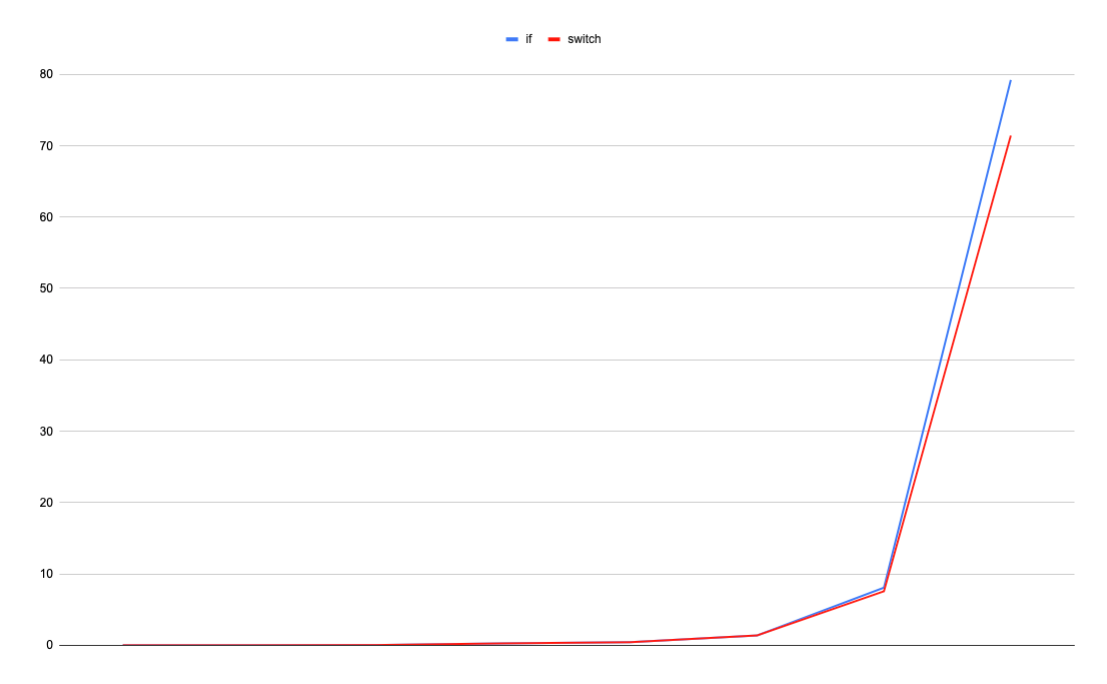
\includegraphics[width=\textwidth]{grafica_if_switch}
                \caption{Gráfica comparativa if-else vs switch}
            \end{figure}

            \newline

            \begin{center}
                \begin{tabular}{ |c|c|c| }
                    \hline
                        iterations & if & switch \\
                        \hline\hline
                        1 & 0.000243 & 0.000270 \\
                        \hline
                        10 & 0.002797 & 0.002485 \\
                        \hline
                        100 & 0.027775 & 0.027261 \\
                        \hline
                        1000 & 0.260075 & 0.261464 \\
                        \hline
                        10000 & 0.431544 & 0.425668 \\
                        \hline
                        100000 & 1.368561 & 1.374575 \\
                        \hline
                        1000000 & 8.070825 & 7.560718 \\
                        \hline
                        10000000 & 79.199539 & 71.409653 \\
                    \hline
                \end{tabular}
            \end{center}

            Como se puede ver en la gráfica, la diferencia no es apreciable hasta las 1000000 iteraciones, pero después
            pasa a casi 8 segundos de diferencia en 10000000 iteraciones. Por esta razón se ha decidido que la función
            utilice la estructura \textit{switch-case}.\newline
            Finalmente, debido a la manera en la que realizan las comprobaciones de qué botones y sensores son
            utilizados, aunque un \textit{switch-case} es más rápido, esta estructura se reserva para la versión del
            programa que reproduce los sonidos leyendo del teclado. En el programa que controla los sensores se utiliza
            una estructura \textit{if-else}.

        % subsubsection if-else vs switch (end)

    % subsection Decisiones (end)

    \subsubsection{Arduino} % (fold)
    \label{ssub:Arduino}

        Para la recepción de las señales del sensor de presión RP c18.3, se plantean dos opciones, se puede utilizar
        la propia Raspberry Pi en la que se ejecuta el programa que maneja los sonidos o una Arduino Nano. En el
        proyecto resultante se utiliza finalmente la Arduino debido a dos razones principales.\newline
        La primera razón es el precio y la escalabilidad, una Raspberry Pi cuesta 39,95\euro{} mientras que una
        Arduino Nano cuesta 10\euro{}. Una Arduino Nano cuenta con menos pines de E/S, pero añadir una placa es más
        barato y sencillo que añadir una placa de Raspberry Pi.\newline
        La segunda razón es la implementación del programa que se encarga de el sensor de presión. En Internet se
        pueden encontrar ejemplos y tutoriales refiriéndose a cómo implementar el sistema en una Arduino, pero no
        es tan fácil encontrar información para hacerlo desde una Raspberry Pi.\newline
        Por estas razones se elige realizar la recepción de las señales del sensor de presión desde la Arduino,
        haciendo el proceso más sencillo y más barato.

    % subsubsection Arduino (end)

% section Diseño (end)

%%%%%%%%%%%%%%%%%%%%%%%%%%%%%%%%%%%%%%%%%%%%%%%%%%%%%%%%%%%%%%%%%%%%%%%%%%%%%%%%%
% Implementación
%%%%%%%%%%%%%%%%%%%%%%%%%%%%%%%%%%%%%%%%%%%%%%%%%%%%%%%%%%%%%%%%%%%%%%%%%%%%%%%%%
\section{Implementación de la propuesta}
\label{sec:Implementacion}

    Poner especial atención al proceso: dificultades y problemas encontrados y cómo se han solucionado

        \subsection{Pads} % (fold)
        \label{sub:Pads}

            Los pads son las superficies que son golpeadas para generar los sonidos. Para este proyecto se han fabricado
            usando madera, cola y gomaeva\cite{GomaEva}. El coste total es de fabricar dos pads es de 3,09\euro{}.
            Comparado con otros productos similares como los de Prologix\cite{practice_pad}, cuyo kit de práctica de 4
            pads cuesta \$224,99, el precio de la solución propuesta en este proyecto es sensiblemente inferior.

        % subsection Pads (end)

        \subsection{Coste y presupuesto} % (fold)
        \label{sub:CosteYPresupuesto}

            tabla con el coste de desarrollo (incluye tu mano de obra... etc.)

        % subsection Coste y presupuesto (end)

        \subsection{Materiales} % (fold)
        \label{sub:Materiales}

            \begin{itemize}
                \item Dos hojas de goma eva: 1,20\euro{}
                \item Tres tablas madera MDF 600x300x10 mm: 7,47\euro{}
                \item Cables protoboard: 2,60\euro{}
                \item Sensor de fuerza Exing c18.3: 5,91\euro{}
                \item Tres sensores de fuerza Exing RP de S40: 50,95\euro{}
                \item Raspberry Pi 3B: 39,95\euro{}
                \item Tarjeta micro SD 8 GB: 5\euro{}
                \item Caja Aukru + cable alimentación: 11,99\euro{}
                \item Dos Arduino Nano: 30,86\euro{} (incluye gastos de envío)
            \end{itemize}

        % subsection Materiales (end)

        \subsection{Tiempo} % (fold)
        \label{sub:Tiempo}

            Para medir el tiempo que ha llevado realizar este trabajo, se ha utilizado la aplicación
            Clockify\cite{clockify}.\newline
            En total se han utilizado 74 horas y 24 minutos.%%%%%%%%%%%%%%%%%%%%%%%%%%%%%%%%%%%%%%%%%%%%%%%%%%%%%%
            %%%%%%%%%%%%%%%%%%%%%%%%%%%%%%%%%%%%%%%%%%%%%%%%%%%%%%%%%%%%%%%%%%%%%%%%%%%%%%%%%%%%%%%%%%%%%%%%%%%%%%
            %%%%%%%%%%%%%%%%%%%%%%%%%%%%%%%%%%%%%%%%%%%%%%%%%%%%%%%%%%%%%%%%%%%%%%%%%%%%%%%%%%%%%%%%%%%%%%%%%%%%%%

        % subsection Tiempo (end)

% section Implementación (end)

 %%%%%%%%%%%%%%%%%%%%%%%%%%%%%%%%%%%%%%%%%%%%%%%%%%%%%%%%%%%%%%%%%%%%%%%%%%%%%%%%%
% Resultados y discusión
%%%%%%%%%%%%%%%%%%%%%%%%%%%%%%%%%%%%%%%%%%%%%%%%%%%%%%%%%%%%%%%%%%%%%%%%%%%%%%%%%
\section{Resultados y discusión}
\label{sec:ResultadosyDiscusion}

    -> Identifica los aspectos éticos y sociales relacionados con la profesión

% section Resultados y discusión (end)

%%%%%%%%%%%%%%%%%%%%%%%%%%%%%%%%%%%%%%%%%%%%%%%%%%%%%%%%%%%%%%%%%%%%%%%%%%%%%%%%%
% Conclusiones
%%%%%%%%%%%%%%%%%%%%%%%%%%%%%%%%%%%%%%%%%%%%%%%%%%%%%%%%%%%%%%%%%%%%%%%%%%%%%%%%%
\section{Conclusiones}
\label{sec:Conclusiones}

    ¿se han satisfecho los objetivos? ¿el porqué? Como se ha visto en \ref{sec:ResultadosDisc}, los o...

    -> Identifica los aspectos éticos y sociales relacionados con la profesión

% section Conclusiones (end)

\bibliographystyle{plain}
\bibliography{referencias}

\end{document}
